\documentclass{article}
\usepackage{amsmath} %%% for the matrix commands
\usepackage{amsthm}
\usepackage{listings}[language=Python, caption=Python example] %%% for software code  highlighting
\usepackage{graphicx} %%% for images
\graphicspath{ {./} }
\newtheorem{definition}{Definition}

\begin{document}

\section{Chapter 2}
In this chapter we will see an end to end example project.
I report the most significative steps:

\begin{itemize}
\item{Look at the big picture}
\item{Get data}
\item{Discover and visualize the data to gain insights}
\item{Prepare the data for Machine learning algorithms}
\item{Select a model and train it}
\item{Fine tune your model}
\item{Present your solution}
\item{Launch, monitor, and maintain your system}
\end{itemize}

Here an explanation of the most significative steps
\begin{definition}
A sequence of data processing components is called a data pipeline.
\end{definition}

\subsection{Look at the big picture:}
You have to ask this questions:
\begin{itemize}
\item{How does the company expect to use and benefit from this model?}
\item{Is it supervised, unsupervised, or Reinforcement Learning? }
\item{Is it a classification task, a regression task, or something else?}
\item{Should you use batch learning or online learning techniques}
\item{Which performance measure should I use?}
\end{itemize}

\subsubsection{Notations}
\begin{itemize}
\item{\textit{m} is the number of instances in the dataset}
\item{$ x^{(i)} $ is a vector of all the features values of the $i^{th}$ instance in the dataset, and $y^{(i)}$ is its label}

\item{\textbf{X} is a matrix containing all the features values of all instances in the dataset (each row is the transpose of the features vector)

$$
   \textbf{X}  = \begin{bmatrix}
             x^{(1)T} \\
             x^{(2)T}\\
             \vdots \\
             x^{(m)T}
         \end{bmatrix}
$$
}
\item{ \textit{h} is your system's prediction function, called a \textit{hypotesis}}

\end{itemize}

The formula of the \textit{Mean Absolute Error} is therefore:
$$MAE(\textbf{X},h) = \frac{1}{m} \displaystyle\sum_{i=1}^{m}  | h(x^{(i)})- y^{(i)})| $$


\subsection{Get data}
It is important to create a test set that is representative of our training set.
Scikit has a relative function:
\begin{lstlisting}
from sklearn.model_selection import train_test_split
\end{lstlisting}
which allow you to pass a dimension of the test set and a seed, so the next time you run it, it will take the same test set (if you continue to change the test set, on the long run you will take the whole trainig set). Be carefull to use a \textit{stratified sampling} allowing to get a representative set of the training set to avoid bias errors.

\subsection{Discover and visualize the data to gain insights}
One try you can give the data is their correlation. To see it, you can use the utils of pandas:
\begin{lstlisting}
corr_matrix = your_df.corr()
corr_matrix["your_attribute"].sort_values(ascending=False)

>>> corr_matrix["perimeter_mean"].sort_values(ascending=False)
perimeter_mean             1.000000
radius_mean                0.997855
concave points_se          0.407217
texture_mean               0.329533
texture_worst              0.303038
smoothness_worst           0.150549
id                         0.073159
fractal_dimension_worst    0.051019
fractal_dimension_se      -0.005523
symmetry_se               -0.081629
texture_se                -0.086761
smoothness_se             -0.202694
fractal_dimension_mean    -0.261477

import matplotlib.pyplot as plt
from pandas.plotting import scatter_matrix

attributes = ["your_attributes", "your_attributes_2", "your_attributes_3",
"your_attributes_4"]
scatter_matrix(your_df[attributes], figsize=(12, 8))
plt.imshow()
\end{lstlisting}

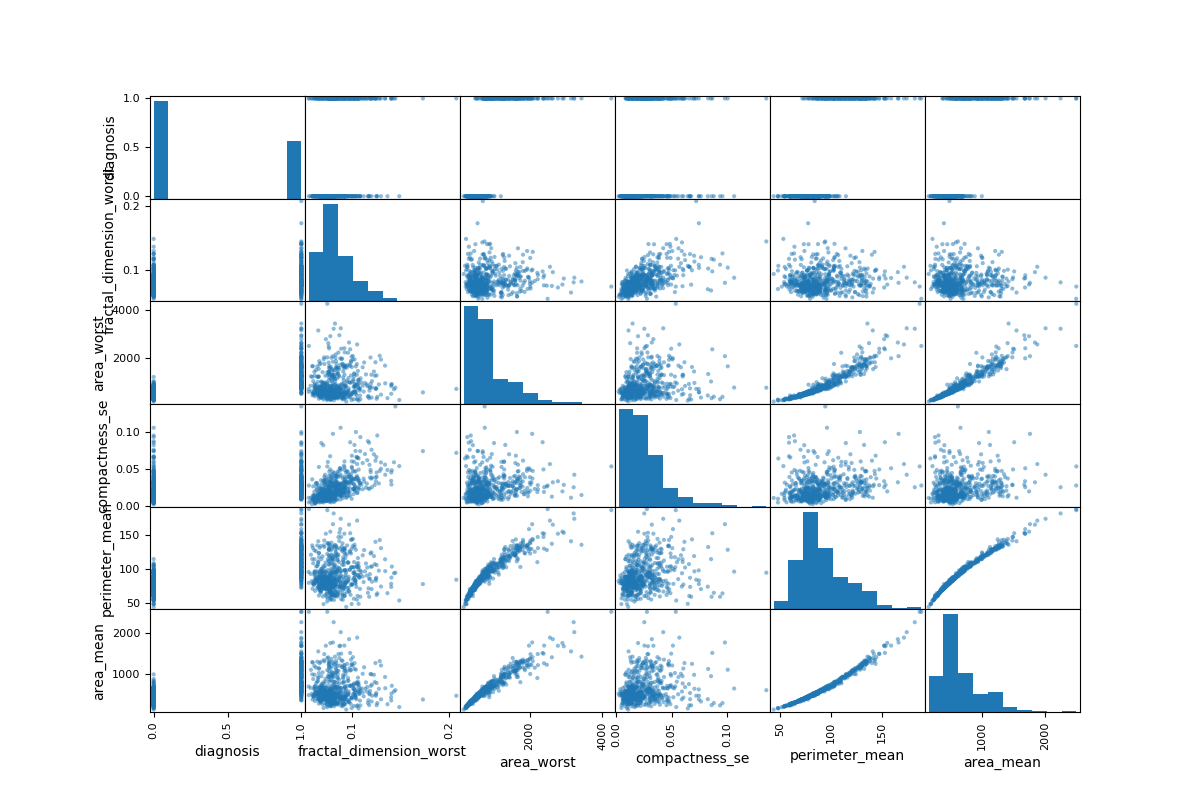
\includegraphics[scale=0.5]{scatter_matrix_example.png}

\subsubsection{Scikit transformers}
To get the full out of correlation, you could have to convert label text to data text, you can do this by \textit{transformers} of the scikit library

\begin{lstlisting}
diagnosis = cancer_cells_df["diagnosis"]
diagnosis_encoded = encoder.fit_transform(diagnosis)
cancer_cells_df["diagnosis"] = diagnosis_encoded
\end{lstlisting}

\subsection{Prepare data for machine learning algorithms}
Data preparation is done with a function in order to make this step reusable.
One step is the handling of missing data (remove it, remove the whole attribute, fill it with zero).

An important possible step is the scaling feature. Scaling is done because some algorithms do not work well with data that has large values and with high variance. The techniques used are standardization and normalization.
Scikit library can handle many transformations with the pipeline class, returning the estimator each time.


\subsection{Select and Train a model}
One method to chose the right model it to test them and evaluate which one perform better. To assess the best model you can use the cross validation feature of scikit learn. The k-fold cross validation split the training set into 10 distinct subsets called folds and evaluates a model 10 times, picking a different fold for evaluation and training on the other 9. The result is 10 evaluation scores.

At least you have to test your model on the test set. Often, the result on this test set will be worse than the result obtained from the cross validation step, because the hyper parameter will be fitted on that set. 

\end{document}
